\subsubsubsubsection{District}
\begin{figure}[h]
\centering
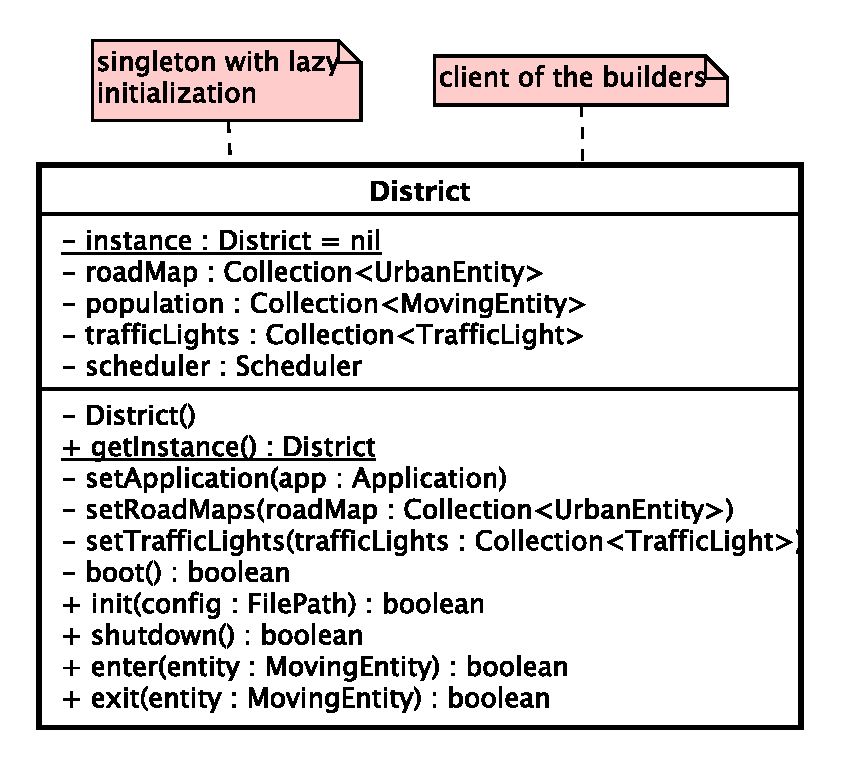
\includegraphics[scale=0.6,keepaspectratio]{images/solution/app/backend/district.eps}
\caption{\pReactive::District}
\label{fig:sd-app-district}
\end{figure}
\FloatBarrier
\begin{itemize}
  \item \textbf{\descr} \\
  It represents the master entity of the application layer. 
  It has the responsibility to boot and shutdown the application layer.
  Ensures the existence of at most one instance of the class, 
  and provides a global point of access to it.
  Uses lazy initialization, hence no class instance is created 
  or stored until one is first requested.
  It is a singleton because the application layer needs 
  only one master entity.
  \item \textbf{\attrs}
  \begin{itemize}
    \item \texttt{\underline{instance : District = nil}} \\
    A static attribute that contains the unique instance of \texttt{District}.
    It is initialized to nil.
    \item \texttt{roadMap: Collection<Infrastracture>} \\
    The urban entities of the district\footnote{Note that the name 
    \textit{district} is only a convention, indeed it is possible to have a 
    real district splitted into different logical nodes of the system}
    (i.e. crossroads and streets). 
    \item \texttt{population: Collection<MoveableAgent>} \\
    The urban actors that reside on the district.
    \item \texttt{trafficLights: Collection<TrafficLight>} \\
    The traffic lights of the district.
    \item \texttt{scheduler: Scheduler} \\
    The scheduler of agent actions.
  \end{itemize}
  \item \textbf{\ops}
  \begin{itemize}
    \item \texttt{District()} \\
    Private and unique constructor because the class has the exclusive 
    responsability for instancing it.
    \item[+] \texttt{\underline{getInstance() : Scheduler}} \\
    Static method lets clients access the unique instance 
    of \texttt{Scheduler}. At the first invocation, it is responsible 
    for creating the instance.
    \item \texttt{setRoadMap(roadMap : Collection<Infrastracture>)} \\
    Sets the urban entities the district includes.
    \item \texttt{setTrafficLights(trafficLights : Collection<TrafficLight>)}
    Sets the traffic lights of the district.
    \item \texttt{boot() : boolean} \\
    Boots the application layer running all the active entities of the 
    district (urban actors and traffic lights).
    Returns true if the process completes neatly, false otherwise. 
    This method is internally used by init.
    \item[+] \texttt{init(config: FilePath) : boolean} \\
    Creates and boots all the entities of the district according to the 
    configuration file. Attaches each crossroads to the relative traffic light
    if specified so in the configuration file. 
    Returns true if the process completes neatly, false otherwise.
    \item[+] \texttt{shutdown() : boolean} \\
    Terminates the district. Returns true if the process completes neatly,
    false otherwise.
    \item[+] \texttt{enter(agent: MoveableAgent) : boolean} \\
    Notifies the district to add a new urban actor to the population.
    Returns true if the process completes neatly, false otherwise.
    \item[+] \texttt{exit(agent: MoveableAgent) : boolean} \\
    Notifies the district to pass a urban actor from the roadMap to the 
    application layer interface which communicates to the middleware layer.
    Returns true if the process completes neatly, false otherwise.
  \end{itemize}
\end{itemize} 
